\section{Categorical Distributions from Densities}  

Often it is useful to find representative patterns (clusters) from sets of
categorical data. These clusters can in turn be considered categories of the
groupings of quantiative data and the cluster membership yields the
distribution of these categories. 

%% PCP's can go here too - relative widths of bands of colors == relative
%% distributions of categories

\begon{figure}
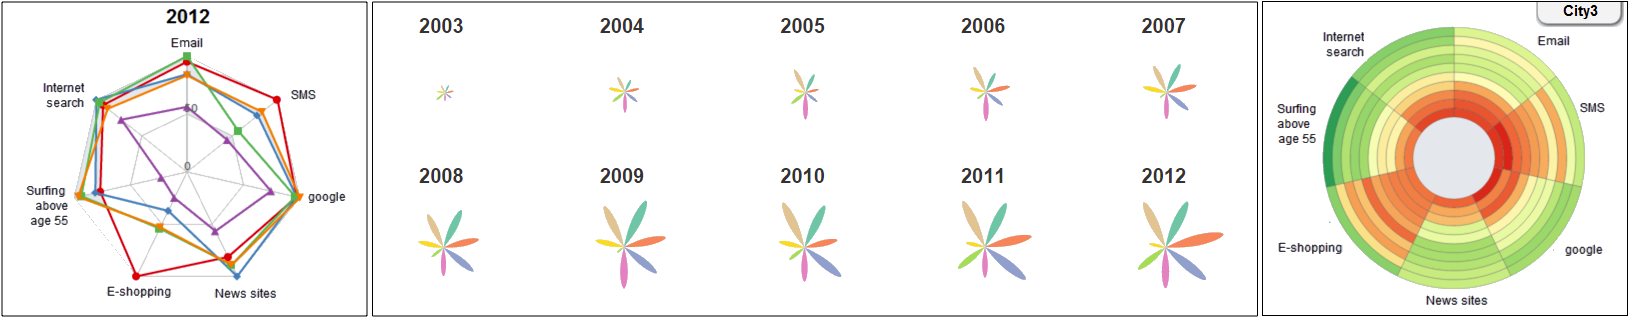
\includegraphics{radial}
\caption{Figrue from \cite{Albo_Bak_}. Rader chart, flower chart, and circle
  charts}
\label{fig:radial}
\end{figure}
Radial visualizations can also be used to show representative
categories from multivariate vectors. For example, as seen in figure~\ref{fig:radial}
rader plot, the clusterings of the area types indicates general categories for
the data, and the number of areas in each cluster indicates the relative
frequency. Flower charts can also be grouped to find these relative
categories, as can the rings in a circle chart. 

